
%%%%%%%%%%%%%%%%%%%%%%%%%%%%%%%%%%%%%%%%%%%%%%%%%%%%
\begin{frame}{Upper bounds -- Convex Cover [skip]}
    \small
    \begin{tcolorbox}[title=Convex cover (informal),colback=green!5!white,colframe=green!50!black]
        Let $\tilde{x}_f \approx \argmin_{x\in \cK} f(x)$. Define $N(\cF, \epsilon)$ to be the smallest number $N$ such that there exists $\{\cF_1,\ldots,\cF_N\}$
        such that:
        \begin{itemize}
            \item \textit{Closure:} $\cF_k$ is a subset of $\cF$ and $\conv(\cF_k) \subset \cF$.
            \item \textit{Common near-minimiser:} There exists an $x_k \in \cK$ such that $\norm{\tilde x_f - x_k} \leq \epsilon$ for all $f \in \cF_k$.
            \item \textit{Approximation:} For all $f \in \cF$ there exists a $k \in [N]$ and $g \in \cF_k$ such that $\norm{f - g}_\infty \leq \epsilon$
                  and $\norm{\tilde x_f - x_k} \leq \epsilon$.
        \end{itemize}
    \end{tcolorbox}
    \begin{tcolorbox}[title=Proposition 2 -- Convex covering number ,colback=blue!5!white,colframe=blue!50!black]
        We have
        \[
            \{N(\cF_{\pb\pl\pr\pm}, \epsilon)\;,\; N(\cF_{\pb\pl}, \epsilon)\} \subset O\left(d\log\left(\frac{\diam(\cK)}{\epsilon}\right)\right)\,.
        \]
    \end{tcolorbox}
\end{frame}
\begin{frame}{Upper bounds -- IR bound in 1-D}
    \small
    \begin{tcolorbox}[title=Theorem 6 -- IR bound for 1-D,colback=blue!5!white,colframe=blue!50!black]
        Suppose that $d = 1$ and $\alpha \in (0,1)$. Then $(\alpha, 10^4 \ceil{\log(1/\alpha)}) \in \IR(\cF_{\pb\pl})$.
    \end{tcolorbox}
    \textbf{Proof.}
    We use our decomposition lemma with
    \begin{align*}
        \cF_i & = \begin{cases}
                      \{f : \bar f(x_f) - f(x_f) \leq \alpha \}                                                  & \text{if } i = 0          \\
                      \{f : \bar f(x_f) - f(x_f) \in (\alpha 2^{|i|-1}, \alpha 2^{|i|}],\, x_f \geq x_{\bar f}\} & \text{if } i > 0          \\
                      \{f : \bar f(x_f) - f(x_f) \in (\alpha 2^{|i|-1}, \alpha 2^{|i|}],\, x_f < x_{\bar f}\}    & \text{if } i < 0      \,,
                  \end{cases}
    \end{align*}
    and the proof is done through Prop 5 if we show
    \uncover<1-3>{
        \only<1-1>{
            \begin{align*}
                \sup_{f \in \cF_i} \left(\bar f(x_f) - f_\star\right)
                \leq
                \epsilon_i
                \leq
                \alpha + \sqrt{230\inf_{f_1,f_2, f_3,f_4 \in \cF_i} \sum_{j,l \in \pair(4)} (f_j(x_{f_l}) - \bar f(x_{f_l}))^2} \,,
            \end{align*}}
        \only<2-2>{
            \begin{align*}
                \sup_{f \in \cF_i} \left(\bar f(x_f) - f_\star\right)
                \underbrace{\leq}_{immediate}
                \epsilon_i
                \leq
                \alpha + \sqrt{230\inf_{f_1,f_2, f_3,f_4 \in \cF_i} \sum_{j,l \in \pair(4)} (f_j(x_{f_l}) - \bar f(x_{f_l}))^2} \,,
            \end{align*}}
        \only<3-3>{
            \begin{align*}
                \epsilon_i
                \underbrace{\leq}_{\text{remaining...}}
                \alpha + \sqrt{230\inf_{f_1,f_2, f_3,f_4 \in \cF_i} \sum_{j,l \in \pair(4)} (f_j(x_{f_l}) - \bar f(x_{f_l}))^2} \,,
            \end{align*}
        }
    }
    for all $i$ show that with $\epsilon_i = \alpha2^{|i|}$.
\end{frame}
\begin{frame}{Upper bounds -- IR bound in 1-D}
    \small
    How does it look like?
    \begin{align*}
        \cF_i & = \begin{cases}
                      \uncover<1->{\{f: \bar f(x_f) - f(x_f) \leq \alpha \}                                                  & \text{if } i = 0}          \\
                      \uncover<3->{\{f: \bar f(x_f) - f(x_f) \in (\alpha 2^{|i|-1}, \alpha 2^{|i|}],\, x_f \geq x_{\bar f}\} & \text{if } i > 0}          \\
                      \uncover<3->{\{f: \bar f(x_f) - f(x_f) \in (\alpha 2^{|i|-1}, \alpha 2^{|i|}],\, x_f < x_{\bar f}\}    & \text{if } i < 0      \,,}
                  \end{cases}
    \end{align*}
    \begin{figure}[h!]
        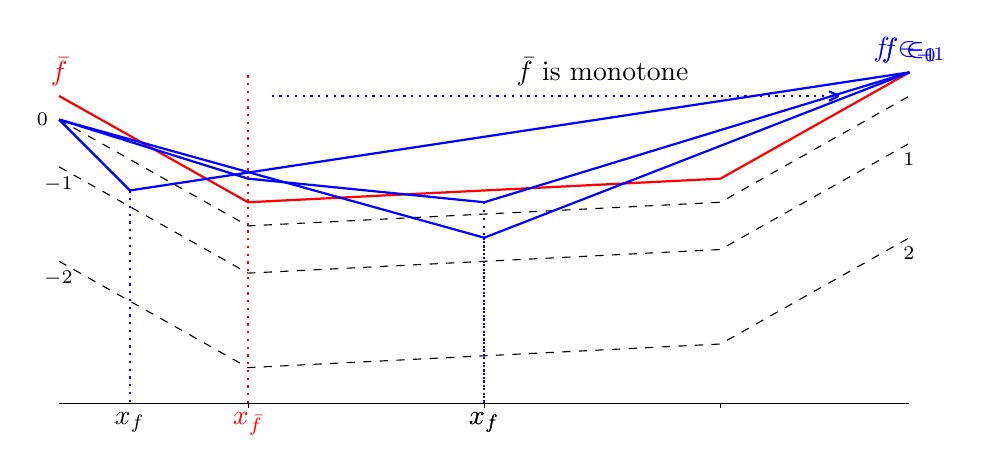
\begin{tikzpicture}[scale=3]
            % bar f
            \draw[thick, red] (-1.8, 1.3) -- (-1,0.85) --(1,0.95) -- (1.8,1.4);
            \node[anchor=south] at (-1.8,1.3) {\textcolor{red}{$\bar f$}};

            %\cF_0
            \uncover<1->{
                \draw[dashed] (-1.8, 1.2) -- (-1,0.75) -- (1,0.85) -- (1.8,1.3);
                \node[anchor=east] at (-1.8,1.2) {$\cF_0$};}

            %f_0
            \uncover<2-2>{
                \draw[thick, blue] (-1.8, 1.2) -- (-1,0.95) --(0,0.85) -- (1.8,1.4);
                \node[anchor=south] at (1.8,1.4) {\textcolor{blue}{$f\in \cF_0$}};
                \draw[thick, blue, dotted] (0,0.85) -- (0,0);
                \node[anchor=north] at (0,0) {$x_f$};
            }

            \uncover<3->{
                \draw[dashed] (-1.8, 1) -- (-1,0.55) -- (1,0.65) -- (1.8,1.1);
                \node[anchor=north] at (-1.8,1) {$\cF_{-1}$};
                \node[anchor=north] at (1.8,1.1) {$\cF_{1}$};
            }

            %vertical
            \uncover<4->{
                \node[anchor=north] at (-1, 0) {\textcolor{red}{$x_{\bar{f}}$}};
                \draw[thick, dotted, red] (-1, 0) -- (-1,1.4);}

            %f_1
            \uncover<5-5>{
                \draw[thick, blue] (-1.8, 1.2) -- (0,0.7) -- (1.8,1.4);
                \node[anchor=south] at (1.8,1.4) {\textcolor{blue}{$f\in \cF_1$}};
                \draw[thick, blue, dotted] (0,0.7) -- (0,0);
                \node[anchor=north] at (0,0) {$x_f$};
            }

            %f_{-1}
            \uncover<6-6>{
                \draw[thick, blue] (-1.8, 1.2) -- (-1.5,0.9) -- (1.8,1.4);
                \node[anchor=south] at (1.8,1.4) {\textcolor{blue}{$f\in \cF_{-1}$}};
                \draw[thick, blue, dotted] (-1.5,0.9) -- (-1.5,0);
                \node[anchor=north] at (-1.5,0) {$x_f$};
            }

            \uncover<7->{
                \draw[dashed] (-1.8, 0.6) -- (-1,0.15) -- (1,0.25) -- (1.8,.7);
                \node[anchor=north] at (-1.8,0.6) {$\cF_{-2}$};
                \node[anchor=north] at (1.8,0.7) {$\cF_{2}$};
            }

            \uncover<8->{
                \draw[blue, thick, dotted] (-0.9,1.3) -> (1.5,1.3);
                \draw[blue, thick] (1.46,1.32) -> (1.5,1.3);
                \draw[blue, thick] (1.46,1.28) -> (1.5,1.3);
                \node[anchor=south] at (0.5, 1.3) {$\bar{f}$ is monotone};
            }

            %axis
            \draw (-1.8,0) -- (1.8,0);
            \draw (0,0) -- (0,-0.02);
            \draw (1,0) -- (1,-0.02);
            \draw (-1,-0) -- (-1,-0.02);

        \end{tikzpicture}
    \end{figure}
\end{frame}

%%%%%%%%%%%%%%%%%%%%%%%%%%%%%%%%%%%%%%%%%%%%%%%%%%%%

\begin{frame}{Upper bounds -- IR bound in 1-D}
    \small
    \textbf{Back to the proof}
    \begin{align*}
        \cF_i & = \begin{cases}
                      \uncover<1->{\{f: \bar f(x_f) - f(x_f) \leq \alpha \}                                                  & \text{if } i = 0}          \\
                      \uncover<3->{\{f: \bar f(x_f) - f(x_f) \in (\alpha 2^{|i|-1}, \alpha 2^{|i|}],\, x_f \geq x_{\bar f}\} & \text{if } i > 0}          \\
                      \uncover<3->{\{f: \bar f(x_f) - f(x_f) \in (\alpha 2^{|i|-1}, \alpha 2^{|i|}],\, x_f < x_{\bar f}\}    & \text{if } i < 0      \,,}
                  \end{cases}
    \end{align*}
    ... and the proof is done through Prop 5 if we show
    \begin{align*}
        \epsilon_i
        \leq
        \alpha + \sqrt{230\inf_{f_1,f_2, f_3,f_4 \in \cF_i} \sum_{j,l \in \pair(4)} (f_j(x_{f_l}) - \bar f(x_{f_l}))^2} \,,
    \end{align*}
    for all $i$ show that with $\epsilon_i = \alpha2^{|i|}$.

    \uncover<2-3>
    {
        \uncover<2-2>{
            \begin{center}
                \textbf{Which trivially holds for $i=0$ since $\epsilon_0 = \alpha$.}
            \end{center}
        }
        \uncover<3->
        {
            \begin{center}
                \textbf{For $i\neq0$ we can use the monotonicity of $\bar{f}$.}
            \end{center}
        }
    }
\end{frame}

%%%%%%%%%%%%%%%%%%%%%%%%%%%%%%%%%%%%%%%%%%%%%%%%%%%%

\begin{frame}{Upper bounds -- IR bound in 1-D}
    \small
    \textbf{Back to the proof for $i \neq 0$ $( \Rightarrow $ monotone $\bar{f}$)}

    % For $i\neq0$ we can use the monotonicity of $\bar{f}$.
    \begin{itemize}
        \item Only 4 functions are enough to get non-negligible disparity.
        \item The proof follows by contradiction.
              Suppose that $x_1 \leq x_2 \leq x_3 \leq x_4$ and
              \begin{align*}
                  \sum_{j,l \in \pair(4)} (f_j(x_{f_l}) - \bar f(x_{f_l}))^2 < c^2 \epsilon^2 \quad \text{for some }c\,,
              \end{align*}
              which means that all $f_1,f_2,f_3,f_4$ are $\epsilon$ close to $\bar{f}$ at all the points $x_1, x_2, x_3, x_4$.
        \item This has to happen while $\bar{f}(x_j) - f_j(x_j) \leq \epsilon_i$ for all $j\in[4]$.
        \item The convexity of $f_1,f_2,f_3,f_4$ and the convexity+monotonicity of $\bar{f}$ in $[x_1, x_4]$ gives the contradiction.
    \end{itemize}
\end{frame}